%%%%%%%%%%%%%%%%%%%%%%%%%%%%%%%%%%%%%%%%%
% Programming/Coding Assignment
% LaTeX Template
%
% This template has been downloaded from:
% http://www.latextemplates.com
%
% Original author:
% Ted Pavlic (http://www.tedpavlic.com)
% License : CC Attribution-NC-SA 3.0.
% Read LICENSE for more information.
%
% Specially edited for competitive programming problem description
% by koosaga(http://koosaga.com), seungwonpark(http://swpark.me)
%
% GitHub repository for this template (currently(2017.05.21) private) :
% https://github.com/seungwonpark/PS-latex-template
%
%%%%%%%%%%%%%%%%%%%%%%%%%%%%%%%%%%%%%%%%%

\documentclass{article}
\usepackage[hangul]{kotex} % Required for using Korean
\usepackage{fancyhdr} % Required for custom headers
\usepackage{lastpage} % Required to determine the last page for the footer
\usepackage{extramarks} % Required for headers and footers
\usepackage[usenames,dvipsnames]{color} % Required for custom colors
\usepackage{graphicx} % Required to insert images
\usepackage{listings} % Required for insertion of code
\usepackage{courier} % Required for the courier font
\usepackage{lipsum} % Used for inserting dummy 'Lorem ipsum' text into the template
\usepackage{amsthm,amsmath} % Equation typesetting
\usepackage{algorithm, algpseudocode} % algorithm
\usepackage{verbatim} % for commment, verbatim environment
\usepackage{spverbatim} % automatic linebreak verbatim environment
\usepackage{listings} % Required for lstlisting
\lstset{breaklines=true} % Word wrap within listings environment
\lstset{basicstyle = \ttfamily,columns=fullflexible}
\usepackage{hyperref} % Required for using href
\usepackage{pgffor} % Required for using \foreach

\lstset{columns=fullflexible}
\DeclareGraphicsExtensions{.pdf,.png,.jpg}
\usepackage{datetime} % Used for showing version as last modified time
\yyyymmdddate
\usepackage{multicol}
\setlength{\columnseprule}{0.4pt}

% Margins
\topmargin=-0.45in
\evensidemargin=0in
\oddsidemargin=0in
\textwidth=6.5in
\textheight=9.0in
\headsep=0.25in

\linespread{1.1} % Line spacing

%%%%%%%%%%%%%%%%%%%%%%%%%%%%%%%%%%%%%%%%%
% Set up the header and footer
\pagestyle{fancy}
\usepackage{lastpage}
\lhead{19:00-22:00}
\chead{leejseonal ddforces (ryuted for div.1)} % Top center head
\rhead{2019년 1월 6일 일요일} % Top right header
\lfoot{} % Bottom left footer
\cfoot{전체 \pageref{LastPage}쪽 중 \thepage 쪽} % Bottom center footer
%\rfoot{Last modified : \today{} \currenttime}
\def\inputdataname{예제 입력 } % Name of 'input'
\def\outputdataname{예제 출력 } % Name of 'output'
%%%%%%%%%%%%%%%%%%%%%%%%%%%%%%%%%%%%%%%%%

\renewcommand\headrulewidth{0.4pt} % Size of the header rule
\renewcommand\footrulewidth{0.4pt} % Size of the footer rule

\setlength\parindent{0pt} % Removes all indentation from paragraphs

\setcounter{secnumdepth}{0} % Removes default section numbers
\newcounter{homeworkProblemCounter} % Creates a counter to keep track of the number of problems

\newcommand{\iodataNo}[2]{%
	\begin{minipage}{\textwidth}
		\begin{multicols}{2}
			{\inputdataname#2} \\
			\rule{\columnwidth}{1pt}
			\lstinputlisting[language={}]{input/input#1.txt}
			\columnbreak
			{\outputdataname#2} \\
			\rule{\columnwidth}{1pt}
			\lstinputlisting[language={}]{output/output#1.txt}
		\end{multicols}
		\vspace{\baselineskip}
	\end{minipage}

}

%\usepackage{graphicsx}

\begin{document}

\section{유의사항}
대회는 총 6문제이며, 다음과 같이 구성되어 있습니다. 문제의 순서는 난이도 순서와는 무관합니다. \newline

\sf \large
\begin{tabular}{|c l c c c c|}
	\hline
	\# & 제목 & 점수 & 시간 제한 & 메모리 제한 & 서브태스크 여부 \\
	\hline
	A & 필름 & 100 & 2000ms & 512MB & X \\
	B & 편안한 문자열 & 100 & 1000ms & 512MB & X \\
	C & 일해라, 류트! & 100 & 2000ms & 512MB & X \\
	D & 감성 테트리스 & 150 & 1000ms & 512MB & O \\
	E & 잉크를 엎질렀다 & 150 & 1000ms & 512MB & O \\
	F & 고양이 소개팅 & 150 & 4000ms & 1024MB & O \\
	\hline
\end{tabular}

\normalsize
\normalfont

\vspace{1.0cm}

본 파일은 표지와 대회에 대한 설명, 그리고 각 문제에 대한 디스크립션을 담고 있습니다. 이는 참가자의 편의를 위해 제공되었을 뿐, BOJ의 디스크립션과 상이한 부분이 있다면, BOJ의 디스크립션을 참고하시기 바랍니다. 뮨재의 설명이 명확하지 않은 부분이나 기타 질문사항이 있으면 BOJ의 `질문하기'를 활용하시기 바랍니다.\newline

대회는 한국 시각 기준 2019년 1월 6일 일요일 19:00-22:00 동안 진행됩니다.\newline

본 대회에는 높은 순위의 참가자 외에도 다른 많은 참가자를 위한 상품(특별상)이 준비되어 있습니다. 특별상을 시상하는 기준은 사전에 결정되었으며, 대회가 종료된 이후에 공개할 예정입니다.

\vspace{1.0cm}

\begin{center}
	
\includegraphics[scale=0.3]{images/logo.pdf}
	\newline
	출제자: ryute, rdd6584, leejseo
	
	운영자: ryute, rdd6584, leejseo, lawali, mixnuts
\end{center}
\vspace{0.5cm}
\begin{center}
	
\includegraphics[scale=0.5]{images/startlink.png}
	
\includegraphics[scale=0.35]{images/boj.png}
	
	BOJ 대회 플랫폼을 지원해주신 startlink에 감사의 말씀을 전합니다.
\end{center}

\newpage

\section{A. 필름}
고고학자 류트는 유적지 발굴 도중 외계 행성 rdd-6584에 사는 외계인의 흔적으로 보이는 기록을 발견하였다. 류트는 다른 기록과 이 기록을 대조하던 도중 이 기록이 특수 필름에 대한 실험 결과라는 것을 알게 되었다. 기록에 따르면 이 필름은 여러 색이 있으며, 삼원색으로만 구성된다는 것을 알게 되었다. 따라서 필름의 색은 빨간색, 초록색, 파란색의 세 단색광의 유무로 표현 가능하며 총 8가지가 존재하게 된다.

\begin{center}
	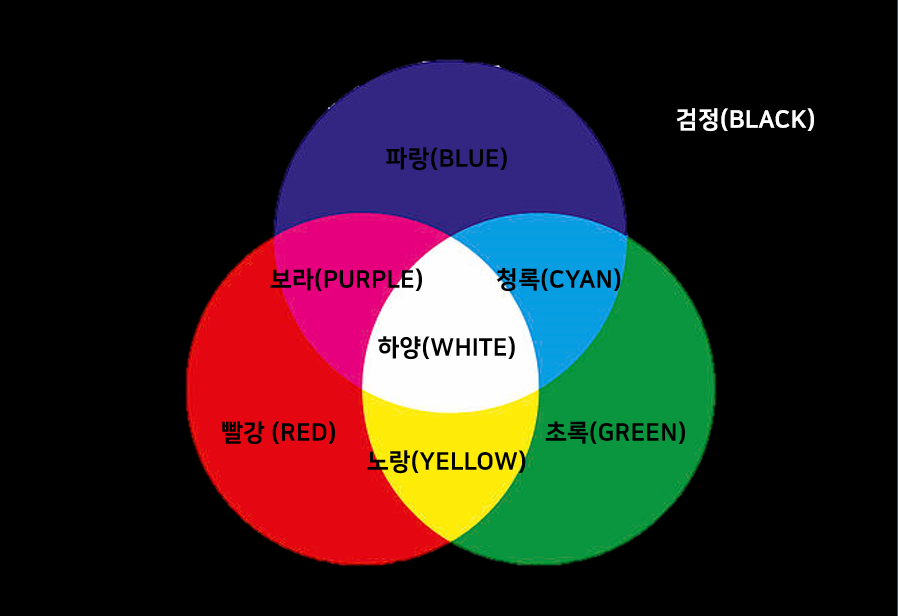
\includegraphics[scale=0.3]{images/01.png}
\end{center}

류트는 이 필름 $n$개에 대해 실험한 실험 기록 $m$개를 찾았다. 필름은 $1$번부터 $n$번까지 번호가 붙여져 있다. 하나의 실험은 두 필름을 겹친 뒤 특정한 파장의 빛을 쏘여 어떤 색깔이 나타나는지 관측하는 것으로 이루어진다. 쏘는 빛은 하나 이상의 단색광의 합으로 이루어진다. 특이하게도 이 필름은 파장에 따라 관측되는 색이 달라진다. 만약 기준보다 높은 파장의 빛을 쏜다면, 그 빛이 가지고 있는 각 단색광마다 두 필름이 모두 그 단색광을 가지고 있어야만 그 단색광을 반사할 것이다. 반대로 기준보다 낮은 파장의 빛을 쏜다면, 그 빛이 가지고 있는 각 단색광마다 두 필름 중 하나 이상이 그 단색광을 가지고 있어야만 그 단색광을 반사할 것이다. 관측되는 색은 반사되는 모든 단색광의 합집합과 같다.\newline

류트는 이 실험 기록이 정말로 외계인이 실험한 기록인지, 아니면 그저 낙서일 뿐인지를 판별하려고 한다. 류트는 다음 조건을 만족하는 실험 기록을 외계인의 실험 기록이라고 하기로 했다.

\begin{itemize}
	\item 모든 실험에는 오류가 없어야 한다. 따라서 파장에 따라 반사되는 빛이 위에 서술된 바와 일치하도록 모든 필름의 색을 정할 수 있는 경우가 하나 이상 존재한다.
\end{itemize}

실험 기록이 주어질 때, 류트는 이 실험 기록이 외계인의 것인지, 또는 낙서일 뿐인지 판단하고 싶다. 류트를 도와주자.

\subsection{입력}
첫 번째 줄에 필름의 개수 $n(1\le n\le 50,000)$과 실험 기록의 개수 $m(1\le m\le 200,000)$이 공백을 사이에 두고 주어진다.\newline

두 번째 줄부터 $m+1$번째 줄 까지 $A$ $B$ $K$ $C_1$ $C_2$ 형태로 실험 기록이 주어진다.\newline

$A$는 첫 번째 필름의 번호, $B$는 두 번째 필름의 번호를 뜻한다. $(1\le A,B \le n)$ $K$는 파장의 높낮이로 기준보다 높으면 \texttt{H}, 낮으면 \texttt{L}이 주어진다. $C_1$과 $C_2$는 각각 쏜 빛과 관측한 빛의 색깔이다. $C_1$과 $C_2$는 표에서 주어진 색 이름 중 하나이다. $C_1$은 조건에 따라 절대 \texttt{BLACK}이 되지 않음에 유의하라. 

\subsection{출력}
외계인의 실험 기록이라면 \texttt{"ALIEN"}을, 그렇지 않다면 \texttt{"THINKINGFACE"}을 출력한다.

\subsection{예제}
% Place input text files at 'input/' directory.
% Format : 'input/input%d.txt'
% Place output text files at 'ouput/' directory.
% Format : 'output/output%d.txt'

\iodataNo{film1}{1}

\textbf{예제 1 설명:} 1번 필름이 노란색, 2번 필름이 파란색, 3번 필름이 노란색이면 조건을 모두 만족한다. 이 조합 외에도 조건을 만족하는 다른 조합이 존재한다. \newline

\iodataNo{film2}{2}

%	% Or, you can use for loop as...
%	\foreach \i in {1, 2, ..., 10}{
%		\iodataNo{\i}
%	}


\textbf{예제 2 설명:} 이 경우에는 조건을 만족하는 조합이 없다. \newline

\newpage

\section{B. 편안한 문자열}
leejseo는 \textbf{할 일 없는 크리스마스}에 괄호 문자열을 가지고 놀고 있었다. 우연하게도 \texttt{"(())"}과 같은 문자열은 좌우 대칭의 형태를 가지고 있지만, 팰린드롬이 아니라는 것을 깨닫게 되었다. leejseo는 비록 이런 문자열이 팰린드롬은 아니지만, 나름대로 의미가 있다 생각했고, \texttt{"(())", ")(", "(()())"}과 같은 문자열을 대칭 문자열이라 부르기로 했다.\newline

즉, 어떤 괄호 문자열(\texttt{'('} 또는 \texttt{')'} 로만 이루어진 문자열)이 대칭 문자열임은 문자들의 순서를 거꾸로 한 후 \texttt{'('}와 \texttt{')'}를 각각 \texttt{')'}와 \texttt{'('}로 바꾼 결과가 자기 자신임을 의미한다. 예를 들어, \texttt{"())(()"}나 \texttt{")("}는 대칭 문자열이며, \texttt{"(("}은 대칭 문자열이 아니다.\newline

leejseo는 대칭 문자열 가운데 올바른 문자열에 더욱 관심이 많았다. 올바른 문자열은 다음과 같이 정의된다:
\begin{itemize}
	\item \texttt{"()"}는 올바른 문자열이다.
	\item $S$가 올바른 문자열일 때, \texttt{'('}+$S$+\texttt{')'}도 올바른 문자열이다.
	\item $S$와 $T$가 올바른 문자열일 때, $S+T$도 올바른 문자열이다.
	\item 이 외의 모든 문자열은 올바른 문자열이 아니다.
\end{itemize}

어떤 문자열이 올바른 문자열인 동시에 대칭 문자열이면 이 문자열은 leejseo를 편-안하게 만드니 편안한 문자열이라 부르자. 어떤 문자열의 부분 문자열이 편안한 문자열이라면, 편안한 부분 문자열이라 부르자. 단, 부분 문자열의 문자들은 원래의 문자열에서 서로 연속한 위치에 있어야 한다. 예를 들어, 문자열 \texttt{"()()"}가 있을 때, \texttt{"(("}는 \texttt{"()()"}의 부분 문자열이 아니며, \texttt{"()()"}의 $1\sim2$번째 문자로 구성된 부분 문자열과 $3\sim4$번째 문자로 구성된 부분 문자열은 모두 \texttt{"()"}이지만 다르게 취급한다.\newline

괄호 문자열이 하나 주어졌을 때, 편안한 부분 문자열의 수를 구해보자.

\subsection{입력}
입력의 첫 줄에 길이가 $1$ 이상 $5,000$ 이하인 괄호 문자열 $S$가 주어진다.

\subsection{출력}
$S$의 편안한 부분 문자열의 수를 출력한다.

\subsection{예제}
\iodataNo{par1}{1}

\textbf{예제 1 설명:} \texttt{"()"} 3개, \texttt{"()()"} 1개, \texttt{"(()())"} 1개로 총 5개의 편안한 부분 문자열이 있다. \newline

\newpage

\section{C. 일해라, 류트!}
디디포스 주식회사에 다니는 류트는 회사의 코딩 테스트를 출제하는 업무를 맡게 되었다. 그는 `고양이 소개팅'이란 문제를 출제했지만, 일하기 귀찮다는 이유로 정해를 짜지 않았고\footnote{실제로 정해를 짜지 않았습니다. 이를 한심하게 여긴 디디가 대신 풀어준 바람에 류트는 풀이도 모릅니다.} 디디에 의해 해고당했다. 일자리를 잃은 류트는 러시아로 이사를 가서 새로운 직업을 찾게 되었다.\newline

우여곡절 끝에 러시아의 화학 공학 기업에서 근무하게 된 류트는 블라디보스토크에서 모스크바로 몇 개의 파이프를 거쳐 여러 화학 약품을 옮기려고 한다. 블라디보스토크에서 모스크바로 화학 약품을 파이프를 통해 수송하려면 총 $M$개의 파이프 $P_1, P_2, \cdots, P_M$을 차례로 거쳐야 한다. 각각의 $i = 1, 2, \cdots, M$ 에 대하여 $P_i$의 길이는 $L_i$이다.\newline

%\begin{center}
%	\includegraphics[scale=0.5]{images/googlemap.png}
	
	
%	\textless 블라디보스토크에서 모스크바를 잇는 파이프를 나타내는 그림\textgreater
%\end{center}

류트가 옮기려는 화학 약품은 총 $N$가지 종류이다. 편의상 이들에 $1, 2, 3, \cdots, N$의 번호를 붙이자. 참고로, 각각의 $1 \le i < j \le N$에 대하여 화학 약품 $i$는 화학 약품 $j$ 보다 먼저 수송되어야 한다.\newline

각각의 $i = 1, 2, \cdots, N$에 대하여 화학 약품 $i$의 점성계수는 $r_i$이다. 점성계수가 $r$인 화학 약품을 길이가 $l$인 파이프로 시각 $t$부터 흘려보내기 시작했다면, 이 화학 약품은 시각 $t+rl$ 직전에 해당 파이프를 완전히 빠져나온다. 다시 말해, $[t, t+rl)$ 동안 해당 파이프를 통과한다.\newline

류트는 여러 화학 약품이 섞일 것을 염려하여, 각각의 $i = 1, 2, \cdots, M$에 대하여 하나의 화학 약품이 $P_i$를 통과한 후, $C_i$ 만큼의 시간이 지나기 이전에는 다른 화학 약품이 $P_i$에 들어오는 일이 없도록 하고자 한다. (이러한 $C_i$들은 류트가 나름의 기준을 가지고 정해놓은 값으로 입력을 통해 주어질 것이다.)\newline

또한, $i = 1, 2, \cdots, M-1$에 대하여 화학 약품이 $P_i$를 빠져 나온 직후에 바로 $P_{i+1}$로 들어가야한다. 다시 말해, 화학 약품이 파이프들을 거쳐 흘러가는 도중에 멈추어서는 안된다.\newline

류트가 시각 $0$부터 시작하여 화학 약품들을 파이프로 흘려보낸다고 하자. 류트는 최소 시간 안에 수송 작업을 완료하고자 한다. 류트가 최소 시간 안에 수송 작업을 완료할 경우 $i = 1, 2, \cdots, N$에 대하여 화학 약품 $i$가 $P_N$을 빠져나오는 시각을 $T_i$라 하자. 이 때, $T_1, T_2, \cdots, T_N$을 구해보자.\newline

\subsection{입력}
입력의 첫 줄에 $N$, $M$이 사이에 공백을 두고 주어진다.

입력이 둘째 줄에 $L_1, L_2, \cdots, L_M$이 사이에 공백을 두고 주어진다.

입력의 셋째 줄에 $C_1, C_2, \cdots, C_M$이 사이에 공백을 두고 주어진다.

입력의 넷째 줄에 $r_1, r_2, \cdots, r_N$이 사이에 공백을 두고 주어진다.

\subsection{출력}
출력의 첫 줄에 $T_1, T_2, \cdots, T_N$을 사이에 공백을 두고 출력한다.

\subsection{제한}
\begin{itemize}
	\item $1 \le N \le 2,000,000$
	\item $1 \le M \le 2,500$
	\item 각각의 $i = 1, 2, \cdots, N$에 대하여 $1 \le r_i \le 100$
	\item 각각의 $i = 1, 2, \cdots, M$에 대하여 $1 \le L_i \le 10,000$, $1 \le C_i \le 100$
	\item 주어지는 입력은 모두 정수이다.
\end{itemize}

\subsection{예제}
\iodataNo{rq1}{1}

\textbf{예제 1 설명:} 화학 약품 1은 $0$초에 $P_1$으로 들어가 $11544(=3\times3848)$초에 $P_1$을 빠져나와 $P_2$로 들어간다. 이후, $20763(=11544+3\times3073)$초에 $P_2$를 빠져나와 $P_3$로 들어가며, 최종적으로 $26727(=20763+3\times1988)$초에 $P_3$을 빠져나온다.\newline

화학 약품 2는 $P_1$으로 들어가는 시각이 $11617(=11544+73)$초 이후여야 하며, $P_2$로 들어가는 시각이 $20830(=20763+67)$초 이후여야 하며, $P_3$로 들어가는 시각이 $26803(=26727+76)$초 이후여야 한다. 이 모두를 만족하는 가장 이른 $P_1$으로 흘려보내기 시작하는 시각은 $11617$초이다. 이 경우, 최종적으로 $P_3$를 빠져나오는 시각은 $198706(=11617+21\times(3848+3073+1988))$초 이다.\newline

같은 방식으로, 류트가 최소 시각 안에 수송 작업을 완료하고자 할 경우, 화학 약품 3은 $502312$초에 $P_3$를 빠져나오게 됨을 쉽게 확인할 수 있다.\newline

\newpage

\section{D. 감성 테트리스}
디디는 $1 \times 4$ `|'자, $4 \times 1$ `$|$'자 모양 블럭으로만 진행되는 테트리스를 하고 있다. 이 테트리스는 어떤 블럭의 떨어질 위치를 정하면 그 위치에서 수직방향으로 떨어지며, 수평방향으로 움직이거나 블럭을 회전시킬 수 없다. 또한 떨어지는 블럭의 아랫면이, 다른 블럭의 윗면 혹은 바닥과 1칸이라도 맞닿는다면, 이 블럭은 떨어지는 것을 멈추고 맞닿는 면 위에 쌓이게 된다.\newline

\begin{center}
	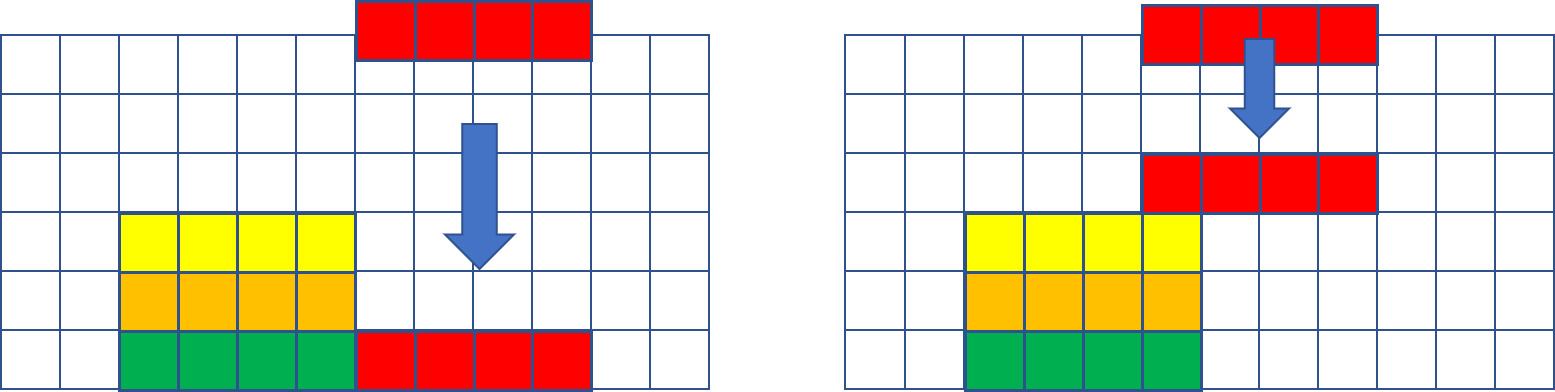
\includegraphics[scale=0.27]{images/02.png}
\end{center}

`이 블럭이 떨어지면 그 밑에 있는 블럭들은 많이 아프겠ㄷr...' 테트리스를 감성으로 하는 디디는 어떤 블럭이 떨어질 때 하중을 받는 블럭의 개수를 구하려고 한다. 떨어지는 블럭의 아랫면과 면을 공유하는 블럭은 하중을 받으며, 하중을 받은 블럭들의 아랫면과 면을 공유하는 블럭들 또한 하중을 받게 된다.\newline

\begin{center}
	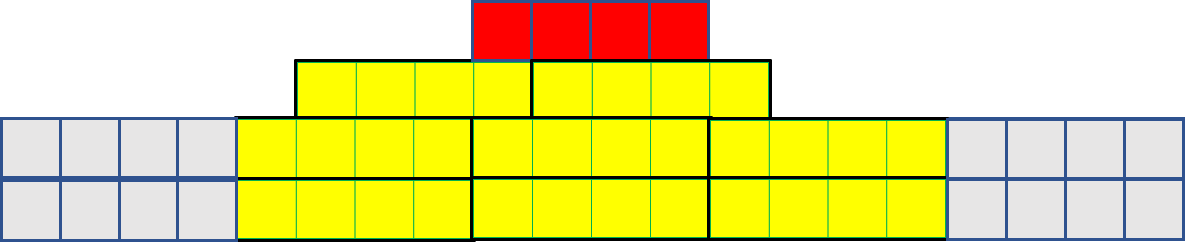
\includegraphics[scale=0.27]{images/03.png}\newline
	\textless 빨간색 블럭은 이번에 떨어뜨린 블럭이며, 노란색 블럭은 이때 하중을 받는 블럭이다.\textgreater
\end{center}

착한 leejseo는 감성이 풍부한 디디를 위해, 디디가 블럭을 떨어뜨릴 때마다 그 블럭의 하중을 받는 블럭의 개수를 구하는 프로그램을 작성하려고 한다. leejseo를 따라서 디디를 도와주자.\newline

\subsection{입력}
첫째 줄에 디디가 떨어뜨린 블럭의 개수 $Q(1 \le Q \le 10^5)$가 주어진다.

둘째 줄부터 $Q$개의 각 줄에는 디디가 떨어뜨린 블럭에 대한 정보가 주어진다.

각 줄은 아래 $2$개 중 하나의 형식을 가지고 있다.

\begin{itemize}
	\item $1$ $a$ : 블럭의 왼쪽 끝 칸이 위치 $a$에 위치하게 `|'자 모양의 블럭을 떨어뜨린다.
	\item $2$ $a$ : 위치 $a$에 `$|$'자 모양의 블럭을 떨어뜨린다.
\end{itemize}
단, $a$는 항상 정수이며 블럭의 어떤 부분도 위치 $1 \sim 400,000$를 벗어나지 않는다.

\subsection{출력}
$Q$개의 각 줄에 디디가 블럭을 떨어뜨릴 때마다 그 블럭의 하중을 받는 블럭의 개수를 출력하라.

\subsection{서브태스크}
\begin{itemize}
	\item 서브태스크1 (34점): 떨어뜨린 블럭의 개수는 $1,000$을 넘지 않는다.
	\item 서브태스크2 (66점): 떨어뜨린 블럭은 전부 `|'자 모양이다.
	\item 서브태스크3 (50점): 추가적인 제약 조건이 없다.
\end{itemize}

\subsection{예제}

\iodataNo{tet1}{1}

\textbf{예제 1 설명:}\newline

\begin{center}
	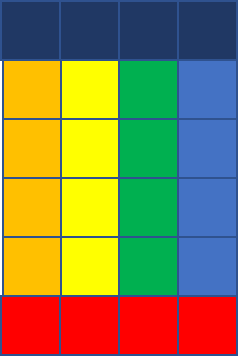
\includegraphics[scale=0.27]{images/04.png}
\end{center}

\iodataNo{tet2}{2}

\textbf{예제 2 설명:}\newline

\begin{center}
	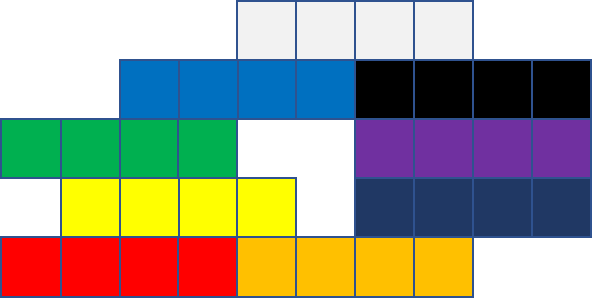
\includegraphics[scale=0.27]{images/05.png}
\end{center}

\newpage

\section{E. 잉크를 엎질렀다}
디디는 알파벳 대문자[\texttt{A-Z}]로 구성된 문자열 $S$에 대해서 $S[1 \sim N]$와 $S$의 부분 문자열 $S[i \sim N]$의 가장 긴 공통 접두사의 길이를 $Z_i$라고 했을 때, 이로 구성된 배열 $Z$를 빠르게 구하는 방법에 대해서 연구하고 있었다. 오랜 공부 끝에 발견한 알고리즘으로 배열 $Z$를 완성시킨 디디는 기쁨의 춤을 추다가 그만 문자열 $S$ 일부에 잉크를 엎질렀다. 그래서 디디는 자신이 만든 배열 $Z$가 올바른 지 확인할 수 없었다. 착한 ryute는 절망한 디디를 위해 문자열 $S$에서 일부 문자가 가려진 문자열 $S^\prime$와 디디가 작성한 배열 $Z$를 이용해서 원본 문자열 $S$를 복원해주려고 한다. 또한, 디디가 만든 배열 $Z$가 올바른지도 대신 확인해주려고 한다. 원본 문자열 $S$로 가능한 경우가 하나라도 있다면 배열 $Z$는 올바른 것으로 간주하고, 그렇지 않다면 올바르지 않은 것으로 간주한다.  ryute를 따라서 디디를 도와주자.

\subsection{입력}
첫째 줄에 문자열 $S$의 길이 $N(1 \le N \le 10^5)$이 주어진다.

둘째 줄에 문자열 $S^\prime$가 주어진다. $S^\prime$는 알파벳 대문자[\texttt{A-Z}]와 \texttt{\#}으로 구성되어 있다. \texttt{\#}은 해당 글자가 잉크에 의해 가려졌다는 것을 의미하며, \texttt{\#}의 개수는 $20$개를 넘지 않는다.

셋째 줄에 디디가 작성한 배열 $Z$의 원소 $Z_i(0 \le Z_i \le N-i+1)$가 순서대로 공백으로 구분되어 주어진다.

\subsection{출력}
디디가 만든 배열 $Z$가 올바르지 않다면 \texttt{THINKINGFACE}를 출력하고, 그렇지 않다면 첫째 줄에 \texttt{YES}, 둘째 줄에 원본 문자열 $S$를 출력하라. 만약, $S$로 가능한 문자열이 여러 개라면 그 중 하나를 출력하라.

\subsection{서브태스크}
\begin{itemize}
	\item 서브태스크1 (23점): $1 \le N \le 3,000$이며, \texttt{\#}의 개수는 1을 넘지 않는다.
	\item 서브태스크2 (77점): $1 \le N \le 3,000$이다.
	\item 서브태스크3 (50점): 추가적인 제약 조건이 없다.
\end{itemize}

\subsection{예제}
\iodataNo{z1}{1}
\iodataNo{z2}{2}
\iodataNo{z3}{3}

\newpage

\section{F. 고양이 소개팅}
류트나라에는 거대한 캣타워가 있다. 캣타워는 루트 있는 트리 구조를 이루고 있다. 따라서 캣타워에는 $1$번부터 $n$번까지 번호가 붙여진 총 $n$개의 보금자리가 있고, 보금자리에 연결된 $n-1$개의 통로가 있다. 캣타워의 맨 위에는 항상 $1$번 보금자리가 있다. 캣타워에 사는 고양이들은 아래쪽 통로를 통해서 살던 보금자리에서 다른 보금자리로 떨어질 수 있다. 단, 고양이들이 통로를 타고 올라갈 수는 없다. 캣타워가 루트 있는 트리 구조이기 때문에, 맨 위 보금자리를 제외하면 임의의 보금자리로 곧바로 떨어질 수 있는 통로는 단 하나 존재한다. 또한 어떤 보금자리에서 다른 보금자리로 떨어질 수 있다면 그 경로는 유일하며, 모든 보금자리는 통로로 이어져 있다. $i$번 보금자리에는 암컷 또는 수컷 고양이가 $c_i$마리 살고 있다. $i$번 보금자리로 곧바로 떨어질 수 있는 통로는 길이가 $d_i$이다. 한 보금자리에서 다른 보금자리로 이동하는 경로의 길이는 한 통로를 두 번 이상 지나지 않으면서 이동할 때 지나게 되는 모든 통로의 길이의 합이 된다.\newline

고양이들은 오늘 단체로 소개팅을 하려고 한다. 고양이들의 소개팅 한 쌍은 암컷 고양이 한 마리와 수컷 고양이 한 마리가 만나서 이뤄진다. 소개팅에 가기 위해서 수컷 고양이는 아래쪽 통로를 통해 이동할 수 있는 보금자리로 뛰어내릴 수 있다. 하지만 공중 곡예비행의 대가라고 불리는 고양이들도 너무 많이 떨어지면 다치기 때문에, $i$번 보금자리에 사는 고양이들은 원래 살던 보금자리로부터 경로의 길이가 $v_i$를 초과하는 정점으로는 뛰어내리지 않기로 했다. 시장 leejseo는 가능한 많은 쌍의 소개팅이 이뤄지길 원한다. leejseo는 어떻게 하면 소개팅 횟수를 최대화 할 수 있을까 고민하다, 당신에게 그 작업을 맡기기로 했다. 캣타워의 구조와 고양이들의 정보가 주어질 때, 성사될 수 있는 소개팅 횟수의 최댓값을 구하시오.

\subsection{입력}
첫 번째 줄에 캣타워 내 보금자리의 개수 $n (1 \le n \le 200,000)$이 주어진다.
 
두 번째 줄에 $1$번 보금자리부터 $n$번 보금자리에 사는 고양이의 수 $c_i (1 \le c_i \le 10^8)$가 차례대로 주어진다.

세 번째 줄에, $1$번 보금자리부터 $n$번 보금자리에 사는 고양이가 떨어질 수 있는 최대 높이 $v_i$($v_i$는 $-1$이거나 $1 \le v_i \le 10^8$)가 차례대로 주어진다. 만약 $v_i$가 $1$ 이상의 정수라면, $i$번 보금자리에는 $c_i$마리의 수컷 고양이가 살고 있다. $v_i$가 $-1$이라면, 그 보금자리에는 $c_i$마리의 암컷 고양이가 살고 있다.

네 번째 줄에 $2$번 보금자리부터 $n$번 보금자리까지 그 보금자리로 곧바로 떨어질 수 있는 보금자리 $a_i (1 \le a_i \le n)$가 차례대로 주어진다.

다섯 번째 줄에 $2$번 보금자리부터 $n$번 보금자리까지 그 보금자리로 곧바로 떨어질 수 있는 통로의 길이 $d_i (1 \le d_i \le 10^8)$가 차례대로 주어진다.    

\subsection{출력}
첫 번째 줄에 성사될 수 있는 소개팅 횟수의 최댓값을 출력하여라.

\subsection{서브태스크}
\begin{itemize}
	\item 서브태스크1 (18점): $2 \le i \le n$인 $i$에 대해 $a_i=i-1$이다.
	\item 서브태스크2 (30점): $1 \le n \le 5,000$이다.
	\item 서브태스크3 (42점): $1 \le i \le n$인 $i$에 대해 $v_i$는 모두 동일하다.
	\item 서브태스크4 (60점): 추가적인 제약 조건이 없다.
\end{itemize}

\subsection{예제}

\iodataNo{c1}{1}

\textbf{예제 1 설명:}\newline
\begin{center}
	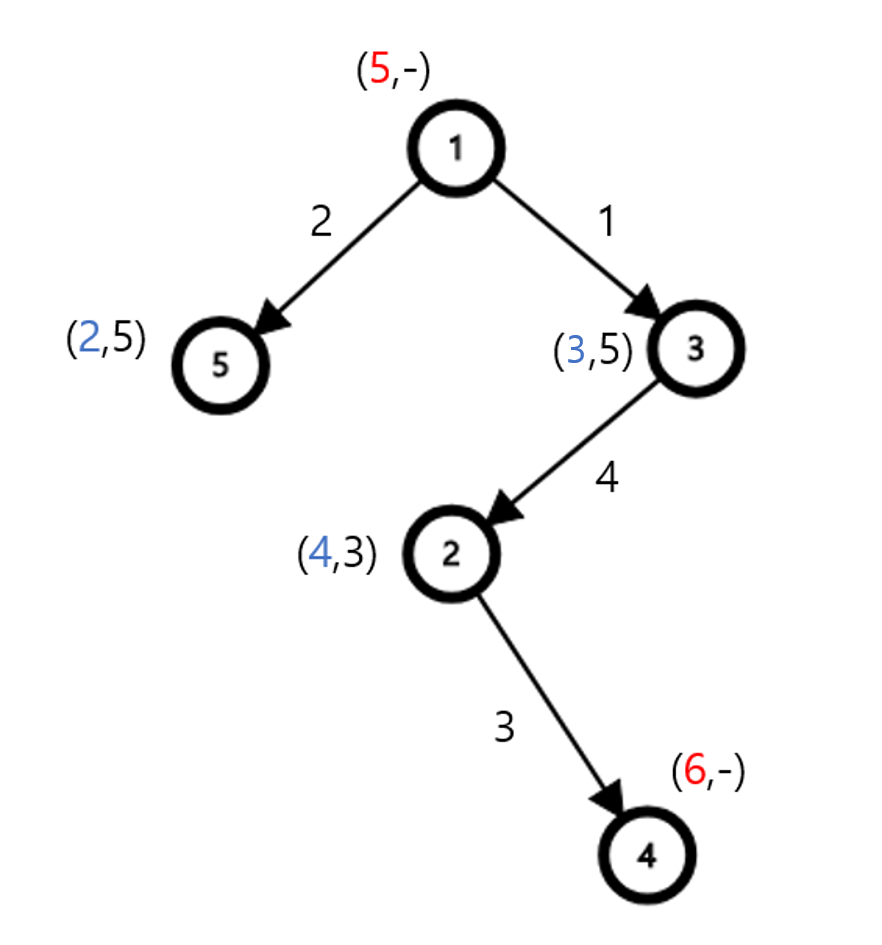
\includegraphics[scale=0.27]{images/06.png}
\end{center}
$2$번 보금자리에서 수컷 고양이 $4$마리가 $4$번 보금자리로 떨어질 수 있다. 이때 성사되는 최대 소개팅 수는 $4$이다. $3$번 보금자리에서 고양이가 뛰어내릴 수 있는 최대 높이는 $5$이기 때문에, $4$번 보금자리까지 뛰어내릴 수 없다.\newline

\vspace{2.5cm}
\begin{center}
	\Large \bf \color{blue}수고하셨습니다.
\end{center}
\end{document}